\documentclass[10pt,a4paper]{article}
\usepackage[utf8]{inputenc}
\usepackage[francais]{babel}
\usepackage[T1]{fontenc}
\usepackage{amsmath}
\usepackage{amsfonts}
\usepackage{amssymb}
\usepackage{graphicx}
\usepackage{hyperref}  % backref linktocpage pagebackref
\author{Antoine Falaize}
\newcommand{\version}{0.2}
\title{\textsc{PyPHS Version \version} \\ Documentation}
% Default fixed font does not support bold face
\DeclareFixedFont{\ttb}{T1}{txtt}{bx}{n}{9} % for bold
\DeclareFixedFont{\ttm}{T1}{txtt}{m}{n}{9}  % for normal

% Custom colors
\usepackage{color}
\definecolor{deepblue}{rgb}{0,0,0.5}
\definecolor{deepred}{rgb}{0.6,0,0}
\definecolor{deepgreen}{rgb}{0,0.5,0}

\usepackage{listings}

% Python style for highlighting
\newcommand\pythonstyle{\lstset{
language=Python,
basicstyle=\ttm,
otherkeywords={self},             % Add keywords here
keywordstyle=\ttb\color{deepblue},
emph={MyClass,__init__},          % Custom highlighting
emphstyle=\ttb\color{deepred},    % Custom highlighting style
stringstyle=\color{deepgreen},
frame=tb,                         % Any extra options here
showstringspaces=false            % 
}}


% Python environment
\lstnewenvironment{python}[1][]
{
\pythonstyle
\lstset{#1}
}
{}

% Python for external files
\newcommand\pythonexternal[2][]{{
\pythonstyle
\lstinputlisting[#1]{#2}}}

% Python for inline
\newcommand\pythoninline[1]{{\pythonstyle\lstinline!#1!}}

%%%%%%% USAGE %%%%%%%
%\begin{document}
%
%\section{``In-text'' listing highlighting}
%
%\begin{python}
%class MyClass(Yourclass):
%    def __init__(self, my, yours):
%        bla = '5 1 2 3 4'
%        print bla
%\end{python}
%
%\section{External listing highlighting}
%
%\pythonexternal{demo.py}
%
%\section{Inline highlighting}
%
%Definition \pythoninline{class MyClass} means \dots
%
%\end{document}
\renewcommand{\vec}[1]{\mathbf{#1}}
\newcommand{\mat}[1]{\mathbf{#1}}
\newcommand{\lab}[1]{\mathtt{#1}}
\newcommand{\op}[1]{\mathrm{#1}}

\newcommand{\Dpar}[2]{\frac{\partial #1}{\partial #2}}
\newcommand{\D}[2]{\frac{\op{d} #1}{\op{d} #2}}
\newcommand{\T}{\intercal}

\renewcommand{\d}{\op{d}}
\newcommand{\vx}{{\vec{x}}}
\newcommand{\vw}{{\vec{w}}}
\newcommand{\vz}{{\vec{z}}}
\newcommand{\vu}{{\vec{u}}}
\newcommand{\vy}{{\vec{y}}}
\newcommand{\vp}{{\vec{p}}}
\newcommand{\vg}{{\vec{g}}}
\newcommand{\vc}{{\vec{c}}}

\newcommand{\vvl}{{\vec{v}_{\lab l}}}
\newcommand{\vvnl}{{\vec{v}_{\lab{nl}}}}

\newcommand{\vfl}{{\vec{f}_{\lab l}}}
\newcommand{\vfnl}{{\vec{f}_{\lab{nl}}}}

\renewcommand{\H}{{\op{H}}}
\newcommand{\Z}[1]{\mat{Z}_{\lab{#1}}}
\newcommand{\J}[1]{\mat{J}_{\lab{#1}}}
\newcommand{\R}[1]{\mat{R}_{\lab{#1}}}
\newcommand{\M}[1]{\mat{M}_{\lab{#1}}}
\newcommand{\N}[1]{\mat{N}_{\lab{#1}}}
\newcommand{\dxH}[1]{\nabla\H_{\lab{#1}}}
\newcommand{\dxHd}[1]{\overline{\nabla}\H_{\lab{#1}}}
\newcommand{\Id}{\mat{I_d}}

\newcommand{\diag}{\operatorname{diag}}

\newcommand{\Q}{\mat{Q}}

\newcommand{\vxl}{\vx_{\lab l}}
\newcommand{\vxnl}{\vx_{\lab{nl}}}
\newcommand{\Hl}{\H_{\lab l}}
\newcommand{\Hnl}{\H_{\lab{nl}}}
\newcommand{\nx}{{n_{\lab{x}}}}
\newcommand{\nxl}{{n_{\lab{xl}}}}
\newcommand{\nxnl}{{n_{\lab{xnl}}}}

\newcommand{\vwl}{\vw_{\lab l}}
\newcommand{\vwnl}{\vw_{\lab{nl}}}
\newcommand{\vzl}{\vz_{\lab l}}
\newcommand{\vznl}{\vz_{\lab{nl}}}
\newcommand{\nw}{{n_{\lab{w}}}}
\newcommand{\nwl}{{n_{\lab{wl}}}}
\newcommand{\nwnl}{{n_{\lab{wnl}}}}

\newcommand{\e}{\mathfrak{e}}
\newcommand{\f}{\mathfrak{f}}
\newcommand{\ve}{\boldsymbol{\e}}
\newcommand{\vf}{\boldsymbol{\f}}

\newcommand{\ny}{n_{\lab{y}}}
\newcommand{\nc}{n_{\lab{y}}}
\renewcommand{\ng}{n_{\lab{g}}}
\newcommand{\np}{n_{\lab{y}}}

\newcommand{\ones}{ \mathbbold{1}}
\newcommand{\zeros}{ \mathbbold{0}}

\newcommand{\RR}{\mathbb{R}}
\newcommand{\CC}{\mathbb{C}}
\newcommand{\NN}{{\mathbb{N}}}
\newcommand{\ZZ}{{\mathbb{Z}}}


%%%%%%
%Fractional Calculus Commandes 
\newcommand{\bmu}{\boldsymbol{\mu}}
\newcommand{\Icx}{{\dot\iota}}
\newcommand{\HH}{{\mathbb{H}}}
\newcommand{\cC}{{\mathcal{C}}}
\newcommand{\EXP}[1]{{\mathrm{e}^{#1}}}
\newcommand{\myvector}[1]{{\mathbf{#1}}}%{{\underline{#1}}}
\newcommand{\Ev}[0]{\myvector{E}}
\newcommand{\Hv}[0]{\myvector{H}}
\newcommand{\Mv}[0]{\myvector{M}}
\newcommand{\Vv}[0]{\myvector{V}}
\newcommand{\Wv}[0]{\myvector{W}}
\newcommand{\herm}[1]{{\overline{#1}^\T}}
\newcommand{\npoles}{{n_\xi}}
\newcommand{\nfreqs}{{n_\omega}}
\newcommand{\fracint}{{\mathcal{I}}}
\newcommand{\fracdiff}{{\mathcal{D}}}

\begin{document}
%
\maketitle
%
\section{Introduction}
%
The python package \pythoninline{pyphs} is dedicated to the treatment of \emph{passive multiphysical systems} in the \emph{Port-Hamiltonian Systems} (PHS) formalism. This formalism structures physical systems into 
%
\begin{itemize}
\item energy conserving parts, 
\item power dissipating parts and 
\item source parts.
\end{itemize}
%

This guarantees a \emph{power balance} is fulfilled, including for numerical \emph{simulations} based on an adapted \emph{numerical method}.   
%

\begin{enumerate}
\item Systems are described by \emph{directed multi-graphs} (\pythoninline{networkx.MultiDiGraph}).
\item The time-continuous port-Hamiltonian structure is build from an \emph{automated graph analysis}.
\item The discrete-time port-Hamiltonian structure is derived from a \emph{structure preserving numerical method}.
\item \LaTeX description code and \textsc{C++} simulation code are automatically generated.
\end{enumerate}
\subsection{Installation}
%
\subsubsection{{Using \texttt{pip}}}
%
It is recommanded to install \pythoninline{pyphs} using \textsc{PyPI} (the \textsc{Python Package Index}). In terminal:
%
\begin{verbatim}
pip install pyphs
\end{verbatim}
%
\subsubsection{{Using \texttt{setuptools}}}
%
\begin{enumerate}
\item Download the sources from the package repository\\ \url{https://github.com/afalaize/pyphs}
\item In a terminal, navigate to the folder that contains the \pythoninline{setup.py} script
\item Install with: 
\begin{verbatim}
python setup.py install
\end{verbatim}
\item To run tests:
\begin{verbatim}
python setup.py test
\end{verbatim}
\end{enumerate}
%
%
\subsubsection{{Using \texttt{Anaconda} (Mac OSX only)}}
%
In terminal:
%
\begin{verbatim}
conda install -c afalaize pyphs
\end{verbatim}
%
\subsection{The PHS formalism}
%
Below is a recall of the Port-Hamiltonian Systems (PHS) formalism.
%
For details, the reader is referred to the \textit{e.g.} the academic reference \cite{falaize2016apassive}.
%
%
We consider systems that can be described by the following time-continuous non-linear state-space representation:
%
%
\begin{equation}
\underbrace{\left(
\begin{array}{c}
\D{\vx}{t}\\
\vw\\
\vy
\end{array}
\right)}_{\vec b}
=
\underbrace{\left(\begin{array}{lll}
\M{xx}&\M{xw} & \M{xy}\\ 
\M{wx}&\M{ww} & \M{wy}\\ 
\M{yx}&\M{yw} & \M{yy}
\end{array}\right)}_{\M{}}
\cdot
\underbrace{\left(
\begin{array}{c}
\dxH{}(\vx)\\
\vz(\vw)\\
\vu
\end{array}
\right)
}_{\vec a}
\end{equation}
%
where 
\begin{equation}
\M{}
=
\underbrace{\left(\begin{array}{lll}
\J{xx}&\J{xw} & \J{xy}\\ 
\J{wx}&\J{ww} & \J{wy}\\ 
\J{yx}&\J{yw} & \J{yy}
\end{array}\right)}_{\J{}}
-
\underbrace{\left(\begin{array}{lll}
\R{xx}&\R{xw} & \R{xy}\\ 
\R{wx}&\R{ww} & \R{wy}\\ 
\R{yx}&\R{yw} & \R{yy}
\end{array}\right)}_{\R{}}
\end{equation}
%
and
%
\begin{itemize}
\item $\J{}:\vx \mapsto \J{}(\vx)$ is a skew-symmetric matrix: $$\J{\alpha\beta}=-\J{\beta\alpha}^\T \mbox{~~for~~} (\alpha, \beta)\in\{\lab x, \lab w, \lab y\}^2,$$
\item $\R{}:\vx \mapsto \R{}(\vx)\succeq 0$ is a positive definite matrix,
\item $\vx: t \mapsto \vx(t)\in\RR^{\nx}$ is the \emph{state vector},
\item $\H:\vx \mapsto \H(\vx)\in \RR_+$ is a \emph{storage function} (convex and positive-definite scalar function with $\H(0)=0$),
\item $\nabla\H:\vx\mapsto\nabla \H(\vx)\in\RR^{\nx}$ denote the gradient of the storage function with the \emph{storage power} $$\op P_\vx = \D{\vx}{t}\cdot \nabla\H(\vx),$$
\item $\vw: t \mapsto \vw(t)\in\RR^{\nw}$ is the \emph{dissipation vector variable},
\item $\vz:\vw \mapsto \vz(\vw)\in \RR^{\nw}$ is a \emph{dissipation function} (with positive definite jacobian matrix and $\vz(0)=0$) for the \emph{dissipated power} $$\op P_\vw = \vw\cdot \vz(\vw) + \vec a\cdot\R{}\cdot\vec a,$$
\item $\vu: t \mapsto \vu(t)\in\RR^{\ny}$ is the \emph{input vector},
\item $\vy: t \mapsto \vy(t)\in\RR^{\ny}$ is the \emph{output vector},
\item  \textbf{the power received \emph{by} the sources \emph{from} the system is} $$\op P=\vu\cdot\vy.$$
\end{itemize}
%

The state is split according to $\vx=(\vxl^\T, \,\vxnl^\T)^\T $ with 
%

\begin{description}
%
\item[$\vxl = (x_1,\cdots,\,x_\nxl)^\T$] the states associated with the quadratic components of the storage function $\Hl(\vxl)=\frac{\vxl\cdot\Q\cdot\vxl}{2}$
%
\item[$\vxnl=(x_{\nxl+1},\cdots,\,x_\nx)^\T$] the states associated with the non-quadratic components of the storage function with $\nx = \nxl+\nxnl$ and $$\H(\vx) = \Hl(\vxl) + \Hnl(\vxnl)$$.\\
%
\end{description}
%

%
The set of dissipative variables is split according to $\vw = (\vxl^\T, \, \vwnl^\T)^\T$ with 
%
\begin{description}
%
\item[$\vwl = (w_1,\cdots,\,w_\nwl)^\T$] the variables associated with the linear components of the dissipative relation $\vzl(\vwl)=\mat{Z}_{\lab l}\,\vwl$
%
\item[$\vwnl=(w_{\nwl+1},\cdots,\,w_\nw)^\T$] the variables associated with the nonlinear components of the dissipative relation $\vznl:\vwnl\mapsto\vznl(\vwnl)\in\RR^{\nwnl}$ with $\nw = \nwl+\nwnl$ and $$ \vz(\vw) = \left(\begin{array}{c}
\mat{Z}_{\lab l}\,\vwl\\
\vznl(\vwnl)
\end{array} \right).$$
%
\end{description}
%

Accordingly, the structure matrices are split as
%
\begin{equation}
\underbrace{\left(\begin{array}{c}
\D{\vxl}{t}\\
\D{\vxnl}{t}\\ \hline
\vwl\\
\vwnl\\ \hline
\vy
\end{array}\right)}_{\vec b}
 = \underbrace{\left(\begin{array}{ll|ll|l}
\M{xlxl}&\M{xlxnl}&\M{xlwl} & \M{xlwnl} & \M{xly}\\ 
\M{xnlxl}&\M{xnlxnl}&\M{xnlwl} &  \M{xnlwnl} & \M{xnly}\\ \hline
\M{wlxl}& \M{wlxnl}& \M{wlwl} & \M{wlwnl} & \M{wly}\\
\M{wnlwl}& \M{wnlxnl}& \M{wnlwl} & \M{wnlwnl} & \M{wnly}\\ \hline
\M{yxl} &\M{yxnl}&\M{ywl} & \M{ywnl} &\M{yy}
\end{array}\right)}_{\M{}}
\cdot
\underbrace{\left(\begin{array}{c}
\Q\cdot\vx\\
\nabla\Hnl(\vxnl)\\ \hline
\mat{Z}_{\lab l}\cdot\vwl\\
\vznl(\vwnl)\\ \hline
\vu
\end{array}\right) }_{\vec a}
\end{equation}
%
\tableofcontents
%
\section{Overview}
%
Below is a list of each module of practical use available in the module \pythoninline{pyphs}, along with a short description. We consider the following instantiation:
%
\begin{python}
# import of (pre-installed) pyphs package:
import pyphs

# instantiate the PortHamiltonianObject:
phs = pyphs.PortHamiltonianObject(label='mylabel')
\end{python}
%
\subsection{The \texttt{symbs} module} Container for all the \textsc{SymPy} symbolic variables (\pythoninline{sympy.Symbol}). 
\begin{description}
%
\item[Attributes] are ordered \emph{list of symbols} associated with the system's vectors components.
%
\begin{description}
\item \pythoninline{phs.symbs.x}: state vector symbols $\vx \in \RR^{\nx}$,
\item \pythoninline{phs.symbs.w}: dissipative vector variable symbols $\vw\in\RR^{\nw}$,
\item \pythoninline{phs.symbs.u}: input vector symbols $\vu\in\RR^{\ny}$,
\item \pythoninline{phs.symbs.y}: output vector symbols $\vy \in \RR^{\ny}$,
\item \pythoninline{phs.symbs.cu}: input vector symbols for connectors $\mathbf{c_u}\in\RR^{\nc}$,
\item \pythoninline{phs.symbs.cy}: output vector symbols for connectors $\mathbf{c_y}\in\RR^{\nc}$,
\item \pythoninline{phs.symbs.p}: Time-varying parameters symbols $\vp\in \RR^{\np}$.
\end{description}
%
\item[Methods]:
%
\begin{description}
%
\item \pythoninline{phs.symbs.dx()}: Returns the symbols associated with the state differential $\d\vx$ formed by appending the prefix $d$ to each symbol in \texttt{x}.
%
\item \pythoninline{phs.symbs.args()}: Return the list of symbols associated with the vector of all arguments of the symbolic expressions (\texttt{expr} module).
%
\end{description}
%
\end{description}
%
\subsection{The \texttt{exprs} module} Container for all the \textsc{SymPy} symbolic expressions \pythoninline{sympy.Expr}associated with the system's functions.
\begin{description}
%
\item[Attributes:] For scalar function (e.g. the storage function $\H$), arguments of \pythoninline{phs.exprs} are \textsc{SymPy} expressions (\pythoninline{sympy.Expr}); for vector functions (e.g. the disipative function $\vz$), arguments are ordered lists of \textsc{SymPy} expressions; for matrix functions (e.g. the Jacobian matrix of disipative function $\vz$), arguments are \pythoninline{sympy.Matrix} objects. Notice the expressions arguments\footnote{Accessed through the \pythoninline{sympy.Expr.free\_symbols} (\textit{e.g.} \pythoninline{phs.exprs.H.free\_symbols} to recover the arguments of the Storage function $\H$).} must belong either to (i) the elements of \pythoninline{phs.symbs.args()}, or (ii) the keys of the dictionary \pythoninline{phs.symbs.subs}.
%
\begin{description}
\item \pythoninline{phs.exprs.H}: storage function $\H\in\RR$,
\item \pythoninline{phs.exprs.z}: dissipative function $\vz\in\RR^{\nw}$,
\item \pythoninline{phs.exprs.g}: input/output gains vector function $\vg \in \RR^{\ng}$,
\end{description}
%
The following expression are computed from the \texttt{exprs.build()} method (see below):
%
\begin{description}
\item \pythoninline{phs.exprs.dxH}: the continuous gradient vector of storage scalar function $\dxH{}(\vx)\in\RR^{\nx}$,
\item \pythoninline{phs.exprs.dxHd}: the discrete gradient vector of storage scalar function $\dxHd{}(\vx, \delta\vx)\in\RR^{\nx}$,
\item \pythoninline{phs.exprs.hessH}: the continuous hessian matrix of storage scalar function (computed as $\nabla\nabla\H(\vx)\in\RR^{\nx\times\nx}$),
\item \pythoninline{phs.exprs.jacz}: the continuous jacobian matrix of dissipative vector function $\nabla\vz(\vw)\in\RR^{\nw\times\nw}$.
\item \pythoninline{phs.exprs.y}: the expression of the continuous output vector function $\vy(\dxH{}, \vz, \vu)\in\RR^{\ny}$,
\item \pythoninline{phs.exprs.yd}: the expression of the discrete output vector function $\overline{\vy}(\dxHd{}, \vz, \vu)\in\RR^{\ny}$,
\end{description}
%
\item[Methods]:
%
\begin{description}
%
\item \pythoninline{phs.exprs.build()}: Build the following system functions as \textsc{SymPy} expressions and append them as attributes to the \pythoninline{phs.exprs} module: \pythoninline{phs.exprs.dxH}, \pythoninline{phs.exprs.dxHd}, \pythoninline{phs.exprs.hessH}, \pythoninline{phs.exprs.jacz}, \pythoninline{phs.exprs.y}, and \pythoninline{phs.exprs.yd}.
%
\item \pythoninline{phs.exprs.setexpr(name, expr)}: Add the \textsc{SymPy} expression \pythoninline{expr} to the \pythoninline{phs.exprs} module, with argument 
\pythoninline{name}, and add \pythoninline{name} to the set of \pythoninline{phs.exprs.\_names}.
%
\item \pythoninline{phs.exprs.freesymbols()}: Return a python set of all the free symbols (\pythoninline{sympy.Symbol}) that appear at least once in all expressions with names in \pythoninline{phs.exprs.\_names}.
\end{description}
%
\end{description}
%
\subsection{The \texttt{dims} module} 
Container for accessors to the system's dimensions. 
%
No attributes should be changed manually. 
%
To split the system into its linear and nonlinear part, use \pythoninline{phs.split_linear()} which organize the system vectors as
%
\begin{equation}
\vx = \left(
\begin{array}{c}
\vx_{\lab{l}} \\
\vx_{\lab{nl}}
\end{array}
\right), \quad \dim(\vx_{\lab{l}}) = 
\end{equation}
%
\begin{description}
%
\item[Attributes:] 
%
\begin{description}
\item \pythoninline{phs.dims.xl}: Number of state vector components associated with a quadratic storage function: $\H_{\lab{l}}(\vx_{\lab{l}}) = \vx_{\lab{l}}^\T\cdot\frac{\Q}{2}\cdot\vx_{\lab{l}}$, and \pythoninline{phs.dims.x()} is equal to \pythoninline{phs.dims.xl + phs.dims.xnl()}.
\item \pythoninline{phs.dims.wl}: Number of dissipative vector variable components associated with a linear dissipative function: $\vz_{\lab{l}}(\vw_{\lab{l}})=\Z{l}\cdot\vw_{\lab{l}}$, and \pythoninline{phs.dims.w()} is equal to \pythoninline{phs.dims.wl + phs.dims.wnl()}.
\end{description}
%
\item[Methods]:
%
\begin{description}
%
\item \pythoninline{phs.dims.x()}: Return the dimension of state vector \pythoninline{len(phs.symbs.x)}.
%
\item \pythoninline{phs.dims.xnl()}: Return the number of state vector components associated with a nonlinear storage function 

\pythoninline{len(phs.symbs.x)}.
%
\item[\texttt{setexpr(name, expr)}]: Add the \textsc{SymPy} expression \texttt{expr} to the \texttt{exprs} module, with argument 
\texttt{name}, and add \texttt{name} to the set of \texttt{exprs.\_names}.
%
\item[\texttt{freesymbols()}]: Retrun a python set of all the free symbols (\texttt{sympy.symbols}) that appear at least once in all expressions with names in \texttt{exprs.\_names}.
\end{description}
%
\end{description}
%
%
%
%
%

\section{Recall on Port-Hamiltonian Systems}
\subsection{\textsc{PHSCore}}
\subsubsection{Attributes}
\begin{description}
\item[•]
\end{description}
\subsubsection{Methods}


\section{Finite dimensionnal dynamical network}
\subsection{\textsc{PHSNetlist}}
\subsection{\textsc{PHSGraph}}

\section{Numerical Methods}
\subsection{PHSNumericalMethod}
\subsection{PHSNumericalMethodStandard}
\appendix
\section{Algorithms}
%
This section details the algorithms actually implemented for 
%
\begin{enumerate}
%
\item the graph analysis and\\
%
\item the different simulation methods
%
\end{enumerate}
%
\subsection{Graph analysis}
%
The graph analysis method that derives the port-Hamiltonian system's differential-algebraic equations from with a given netlist is detailed in the reference \cite{falaize2016apassive}.
%
The algorithm implemented in \textsc{PyPHS} is exactly that in \cite[algorithm 1]{falaize2016apassive}.
%
\subsection{Simulation methods}
%
The discrete gradient method is used in conjunction with the port-Hamiltonian structure to produce a passive-guaranteed numerical scheme (see \cite{falaize2016apassive} for details).
%
In the sequel, quantities are defined on the current time step $\vx\equiv\vx(t_k)$, with $k\in\mathbb{N}_{+}^{*}$.
%
\subsubsection{Split of the linear part from the nonlinear part}
%
The dicrete gradient for the quadratic part of the Hamiltonian is ${\small \nabla\Hl =\frac{1}{2}\,\mat{Q}\, (2\vxl + \delta \vxl)}$ and the discret linear subsystem is
 %
%
\begin{equation}
\begin{array}{rcl}
\mat{D}_{\lab l}^{-1} = \mat{iD}_{\lab l} &=& \left(\begin{array}{ll}
\frac{\Id}{\delta t}&0 \\ 
0 &\Id
\end{array}\right)-\left(\begin{array}{ll}
\M{xlxl}&\M{xlwl} \\ 
\M{wlxl}&\M{wlwl} 
\end{array}\right)\,\left(\begin{array}{ll}
\frac{1}{2}\,\mat{Q}&0 \\ 
0 &\mat{Z}_{\lab l}
\end{array}\right),\\
\underbrace{\left(\begin{array}{c}
\delta \vxl\\
\vwl
\end{array}\right) 
}_{\vec{v}_{\lab l}}
& = &
\underbrace{\mat{D}_{\lab l}\,
\underbrace{\left(\begin{array}{ll}
\M{xlxl}\\ 
\M{wlxl}
\end{array}\right)\,\Q}_{\overline{\N{lxl}}}}_{\N{lxl}}
\, 
\vxl
+
  \underbrace{\mat{D}_{\lab l}\,
\underbrace{\left(\begin{array}{ll}
\M{xlxnl}& \M{xlwnl} \\ 
 \M{wlxnl}& \M{wlwnl} 
\end{array}\right)}_{\overline{\N{lnl}}}}_{\N{lnl}}
\,
\underbrace{\left(\begin{array}{c}
\nabla\Hnl\\
\vznl
\end{array}\right) 
}_{\vec{f}_{\lab{nl}}}
+
  \underbrace{\mat{D}_{\lab l}\,
\underbrace{\left(\begin{array}{l}
 \M{xly}\\ 
 \M{wly}
\end{array}\right)}_{\overline{\N{ly}}}}_{\N{ly}}
\,
\vu
\end{array}
\end{equation}
%
and the nonlinear subsystem is 
%
\begin{equation}
\begin{array}{rcl}
\left(
\begin{array}{cc}
\frac{\Id}{\delta t} & 0 \\
0 & \Id
\end{array}
\right)\underbrace{\left(\begin{array}{c}
\delta \vxnl \\
\vwnl
\end{array}\right) 
}_{\vec v_{\lab{nl}}}
&=&
  \underbrace{\left(\begin{array}{ll}
\M{xnlxnl}& \M{xnlwnl} \\ 
 \M{wnlxnl}& \M{wnlwnl} 
\end{array}\right)}_{\overline{\N{nlnl}}}
\,
\vec{f}_{\lab {nl}}
+
  \underbrace{\left(\begin{array}{l}
 \M{xnly}\\ 
 \M{wnly}
\end{array}\right)}_{\overline{\N{nly}}}
\,
\vu \\
 && +
\underbrace{ \left(\begin{array}{ll}
\M{xnlxl}&\M{xnlwl} \\ 
\M{wnlxl}&\M{wnlwl} 
\end{array}\right)\,\left(\begin{array}{ll}
\frac{1}{2}\,\mat{Q}&0 \\ 
0 &\mat{Z}_{\lab l}
\end{array}\right)}_{\overline{\N{nll}}}
\, 
\vec v_{\lab{l}}
+
\underbrace{\left(\begin{array}{ll}
\M{xnlxl}\\ 
\M{wnlxl}
\end{array}\right)\,\Q}_{\overline{\N{nlxl}}}
\, 
\vxl
\end{array}
\end{equation}
\subsubsection{Presolve numerical nonlinear subsystem}
\begin{equation}
\begin{array}{rcl}
\left(
\begin{array}{cc}
\frac{\Id}{\delta t} & 0 \\
0 & \Id
\end{array}
\right)\,
\vec v_{\lab{nl}} &=& \underbrace{\left(\overline{\N{nlxl}} + \overline{\N{nll}}\,{\N{lxl}}\right)}_{\N{nlxl}}\,\vxl + \underbrace{\left(\overline{\N{nlnl}} + \overline{\N{nll}}\,{\N{lnl}}\right)}_{\N{nlnl}}\,\vec f_{\lab{nl}}\\
&& \underbrace{\left(\overline{\N{nly}}+ \overline{\N{nll}}\,{\N{ly}}\right)}_{\N{nly}}\,\vu
\end{array}
\end{equation}
%
\subsubsection{Algorithm}
\paragraph{Inputs}
\begin{equation}
\begin{array}{rcl}
\mat{iD}_{\lab l} &=& \left(\begin{array}{ll}
\frac{\Id}{\delta t}&0 \\ 
0 &\Id
\end{array}\right)-\left(\begin{array}{ll}
\M{xlxl}&\M{xlwl} \\ 
\M{wlxl}&\M{wlwl} 
\end{array}\right)\,\left(\begin{array}{ll}
\frac{1}{2}\,\mat{Q}&0 \\ 
0 &\mat{Z}_{\lab l}
\end{array}\right) 
\\
\overline{\N{lxl}}
&=&
\left(\begin{array}{ll}
\M{xlxl}\\ 
\M{wlxl}
\end{array}\right)\,\mat Q
\\
\overline{\N{lnl}}
&=&
\left(\begin{array}{ll}
\M{xlxnl} & \M{xlwnl}\\ 
\M{wlxnl} & \M{wlwnl}
\end{array}\right)
\\
\overline{\N{ly}}
&=&
\left(\begin{array}{ll}
\M{xly}\\ 
\M{wly}
\end{array}\right)
\\
\overline{\N{nlnl}}
&=&
\left(\begin{array}{ll}
\M{xnlxnl}& \M{xnlwnl} \\ 
 \M{wnlxnl}& \M{wnlwnl} 
\end{array}\right)
\\
\overline{\N{nll}}
&=&
\left(\begin{array}{ll}
\M{xnlxl}& \M{xnlwl} \\ 
 \M{wnlxl}& \M{wnlwl} 
\end{array}\right)
\,
\left(\begin{array}{ll}
\frac{1}{2}\Q	& 0\\ 
0& \mat Z_\lab l
\end{array}\right)
\\
\overline{\N{nlxl}}
&=&
\left(\begin{array}{ll}
\M{xnlxl}\\ 
 \M{wnlxl}
\end{array}\right)
\,
\Q
\\
\overline{\N{nly}}
&=&
\left(\begin{array}{ll}
\M{xnly}\\ 
 \M{wnly}
\end{array}\right)
\\
\mathcal{J}_{\vec f \lab {nl}}(\vec v_{\lab {nl}})
&=&
\left(\begin{array}{ll}
\mathcal{J}_{\nabla \Hnl}	& 0\\ 
0& \mathcal{J}_{\vznl}
\end{array}\right)
\\
\mat I_{\lab{nl}}
&=&
\left(
\begin{array}{cc}
\frac{\Id}{\delta t} & 0 \\
0 & \Id
\end{array}
\right)
\end{array}
\end{equation}
%
\paragraph{Process}
\begin{equation}
\begin{array}{rcl}
\mat D_{\lab l}&=& \mat{iD}_{\lab l}^{-1}\\
\N{lxl} &=& \mat D_{\lab l}\,\overline{\N{lxl}}\\
\N{lnl} &=& \mat D_{\lab l}\,\overline{\N{lnl}}\\
\N{ly} &=& \mat D_{\lab l}\,\overline{\N{ly}}\\
\N{nlxl} &=& \overline{\N{nlxl}} + \overline{\N{nll}}\,{\N{lxl}}\\
\N{nlnl} &=& \overline{\N{nlnl}} + \overline{\N{nll}}\,{\N{lnl}}\\
\N{nly} &=& \overline{\N{nly}} + \overline{\N{nll}}\,{\N{ly}}\\
\vec c &=& \N{nlxl}\,\vxl + \N{nly}\,\vu \\
\mbox{Iterate}  &:&\vec F_{\lab{nl}}(\vec v_{\lab{nl}})=\mat I_{\lab{nl}}\, \vec v_{\lab{nl}}-\N{nlnl}\,\vec f_{\lab{nl}} - \vec c \\
&&\mathcal{J}_{\vec F_{\lab{nl}}}(\vec v_{\lab{nl}}) 
=
\mat I_{\lab{nl}} - \N{nlnl}\,\mathcal{J}_{\vec f \lab {nl}}(\vec v_{\lab {nl}})\\
& & \vec v_{\lab{nl}} = \vec v_{\lab{nl}}-\mathcal{J}^{-1}_{\vec F_{\lab{nl}}}(\vec v_{\lab{nl}}) \,\vec F_{\lab{nl}}(\vec v_{\lab{nl}})\\
\vec v_{\lab{l}} &=& \N{lxl}\,\vxl +\N{lnl}\,\vec f_{\lab{nl}} + \N{ly}\,\vu\\
\vy & = &\M{yxl}\,\nabla \Hl + \M{yxnl}\,\nabla \Hnl\M{ywl}\,\mat Z_{\lab l}\,\vwl + \M{ywnl}\,\vznl + \M{yy}\,\vu\\
\vx & = &\vx+ \delta \vx
\end{array}
\end{equation}

\begin{eqnarray}
\vy & = &\M{yxl}\,\nabla \Hl + \M{yxnl}\,\nabla \Hnl\M{ywl}\,\mat Z_{\lab l}\,\vwl + \M{ywnl}\,\vznl + \M{yy}\,\vu\\
&=& \M{yxl}\,\nabla \Hl + \M{yxnl}\,\nabla \Hnl\M{ywl}\,\mat Z_{\lab l}\,\vwl + \M{ywnl}\,\vznl + \M{yy}\,\vu\\
\end{eqnarray}

\subsection{Realizability solver}
%
\textbf{Connections\\}
\paragraph{Serial}
$\sum_{n=1}^N e_n = 0$, \\
$f_1 = \cdots = f_N = \phi$ (variable commune)
\paragraph{parallel}
$\sum_{n=1}^N f_n = 0$,\\
 $e_1 = \cdots = e_N = \phi$ (variable commune)

\textbf{Storage}
\paragraph{Realizable}
$$\left\{ \begin{array}{rcl}
\phi = u =\D{}{t} x &=& \D{x_1}{t} =\cdots = \D{}{t}{x_N} \\
y = \dxH(x)&=& \sum_{i=1}^N\dxH{}{}_{}i(x_i) \end{array}\right.$$
alors $ x = x_1 = x_2 $ et $\H(x) = \left(\sum_{i=1}^N \H_i\right)(x)$
\paragraph{Non-Realizable}
$$\left\{ \begin{array}{rcl}
\phi = u =\dxH (x)& =& \dxH{}{}_{}{}1(x_1) =\cdots = \dxH{}{}_N(x_N),\\
y=  \D{}{t}{x} & =& \sum_{i=1}^N \D{}{t}{x_i} \end{array}\right.$$
alors $ x =\sum_{i=1}^N x_i $ et $\H(x) = \left(\sum_{i=1}^N H_i \dxH{}{}_i^{-1} G \right) (x) $ \\
avec $G^{-1}(x) = \sum_{i=1}^N\dxH{}{}_i(x_i)$


\textbf{Dissipatives}
\paragraph{Realizable} 
$$\left\{ \begin{array}{rcl}
\phi = u =w &=& w_1 =\cdots = w_N ,\\
y =z(w)&= &\sum_{i=1}^N z_i(x_i) 
\end{array}\right.$$
\paragraph{Non-Realizable}
$$\left\{ \begin{array}{rcl}
\phi = u =z(w) &=& z_1(w_1) =\cdots = z_N(w_N) ,\\
y = w &=& \sum_{i=1}^Nw_i\end{array}\right.$$
alors $ w =\sum_{i=1}^N w_i=\left(\sum_{i=1}^N z^{-1}_i\right)(\phi) $ et $z^{-1}(\phi) = w\Rightarrow z(w) =  \left(\sum_{i=1}^N z_i\right)^{-1}(w)$


\section{Connectors: Gyrators and Transformers}
A connector is set of two edges ($e_1$, $e_2$), the efforts and flux of which are coupled depending on the connector's type.
\subsection{Gyrator}
%
\begin{figure}
\centering
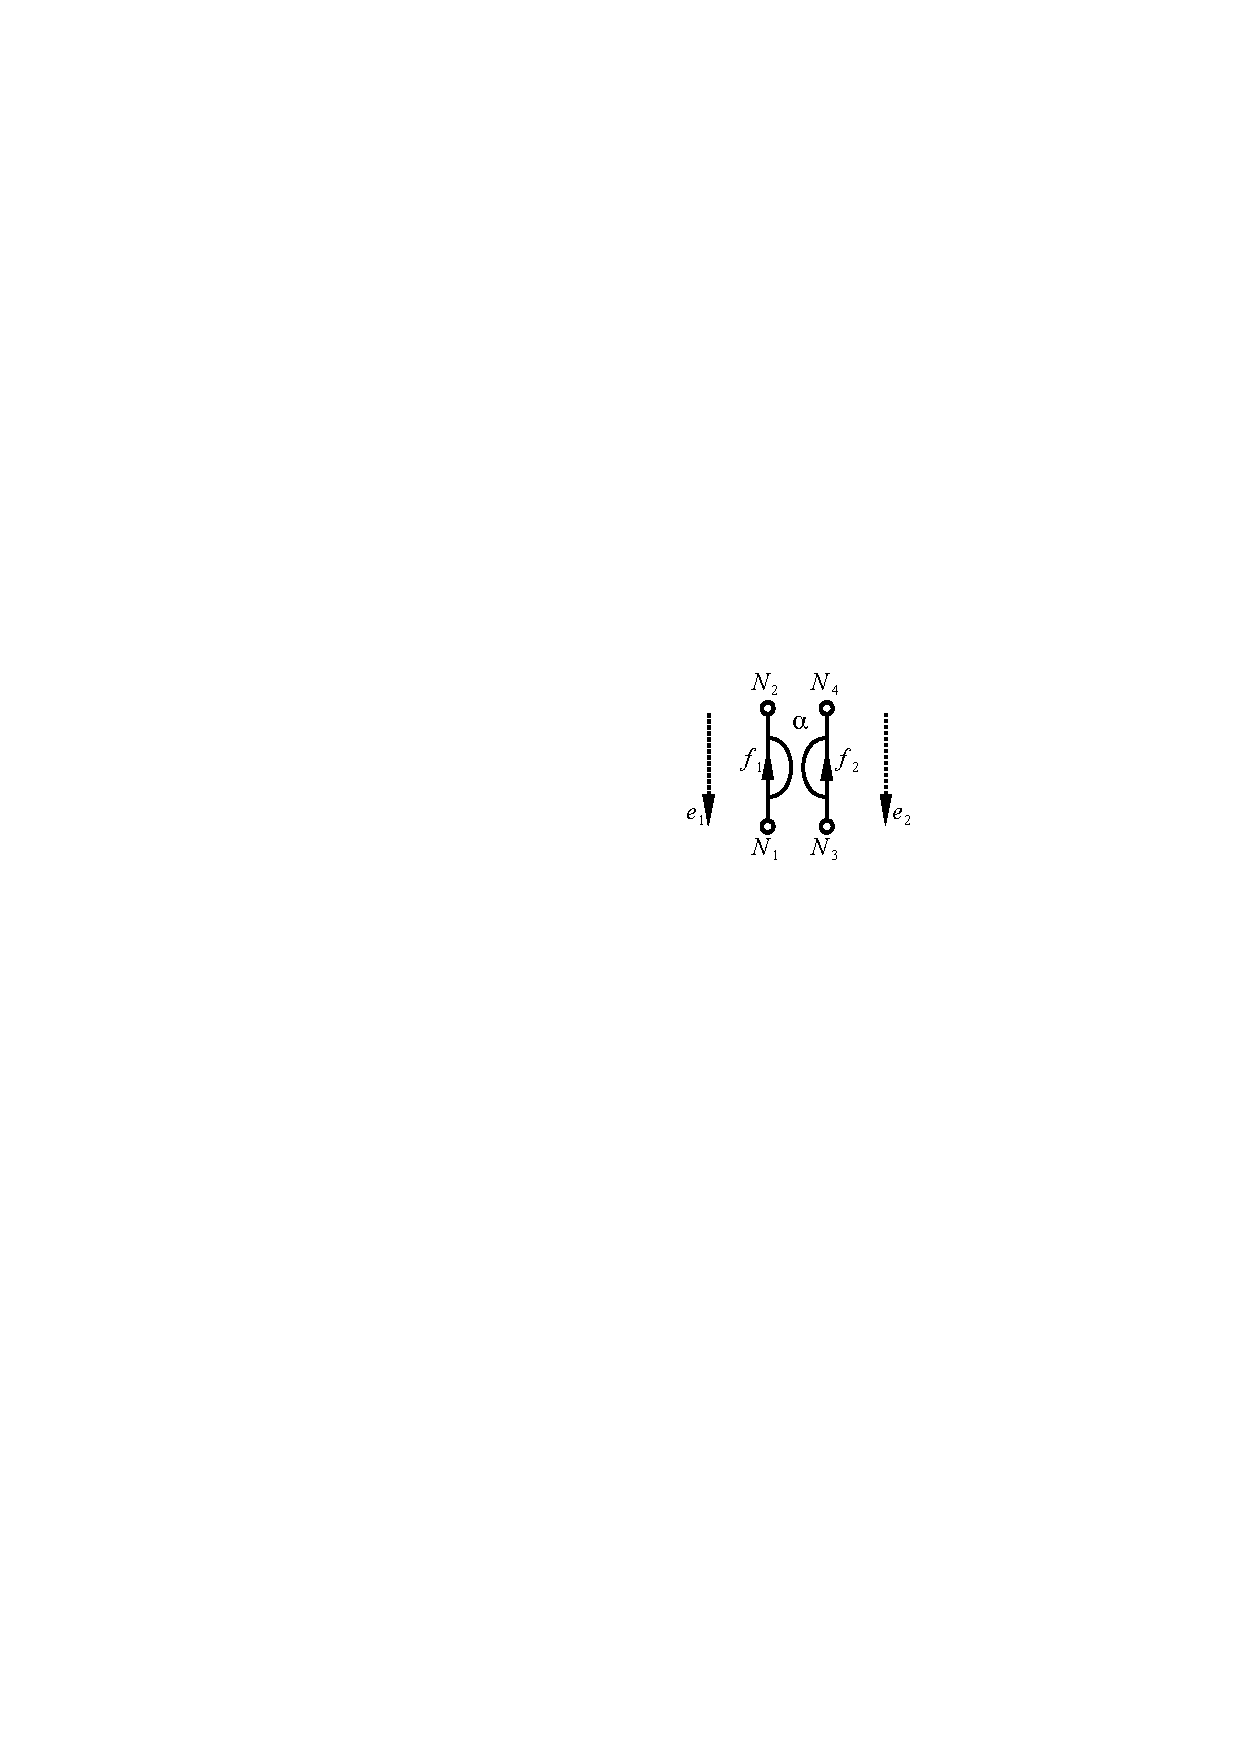
\includegraphics[width=0.3\linewidth]{figures/gyrator_scematic.pdf} 
\caption{Scematic and conventions for the gyrator.}
\end{figure}
%
\paragraph{Constitutive relations}
$$
\left(
\begin{array}{c}
\e_1\\
\e_2
\end{array}
\right)
=
\left(
\begin{array}{rr}
0 & -\alpha \\
+ \alpha  & 0
\end{array}
\right)
\cdot
\left(
\begin{array}{c}
\f_1\\
\f_2
\end{array}
\right)
$$
\subsection{Transformer}
\begin{figure}
\centering
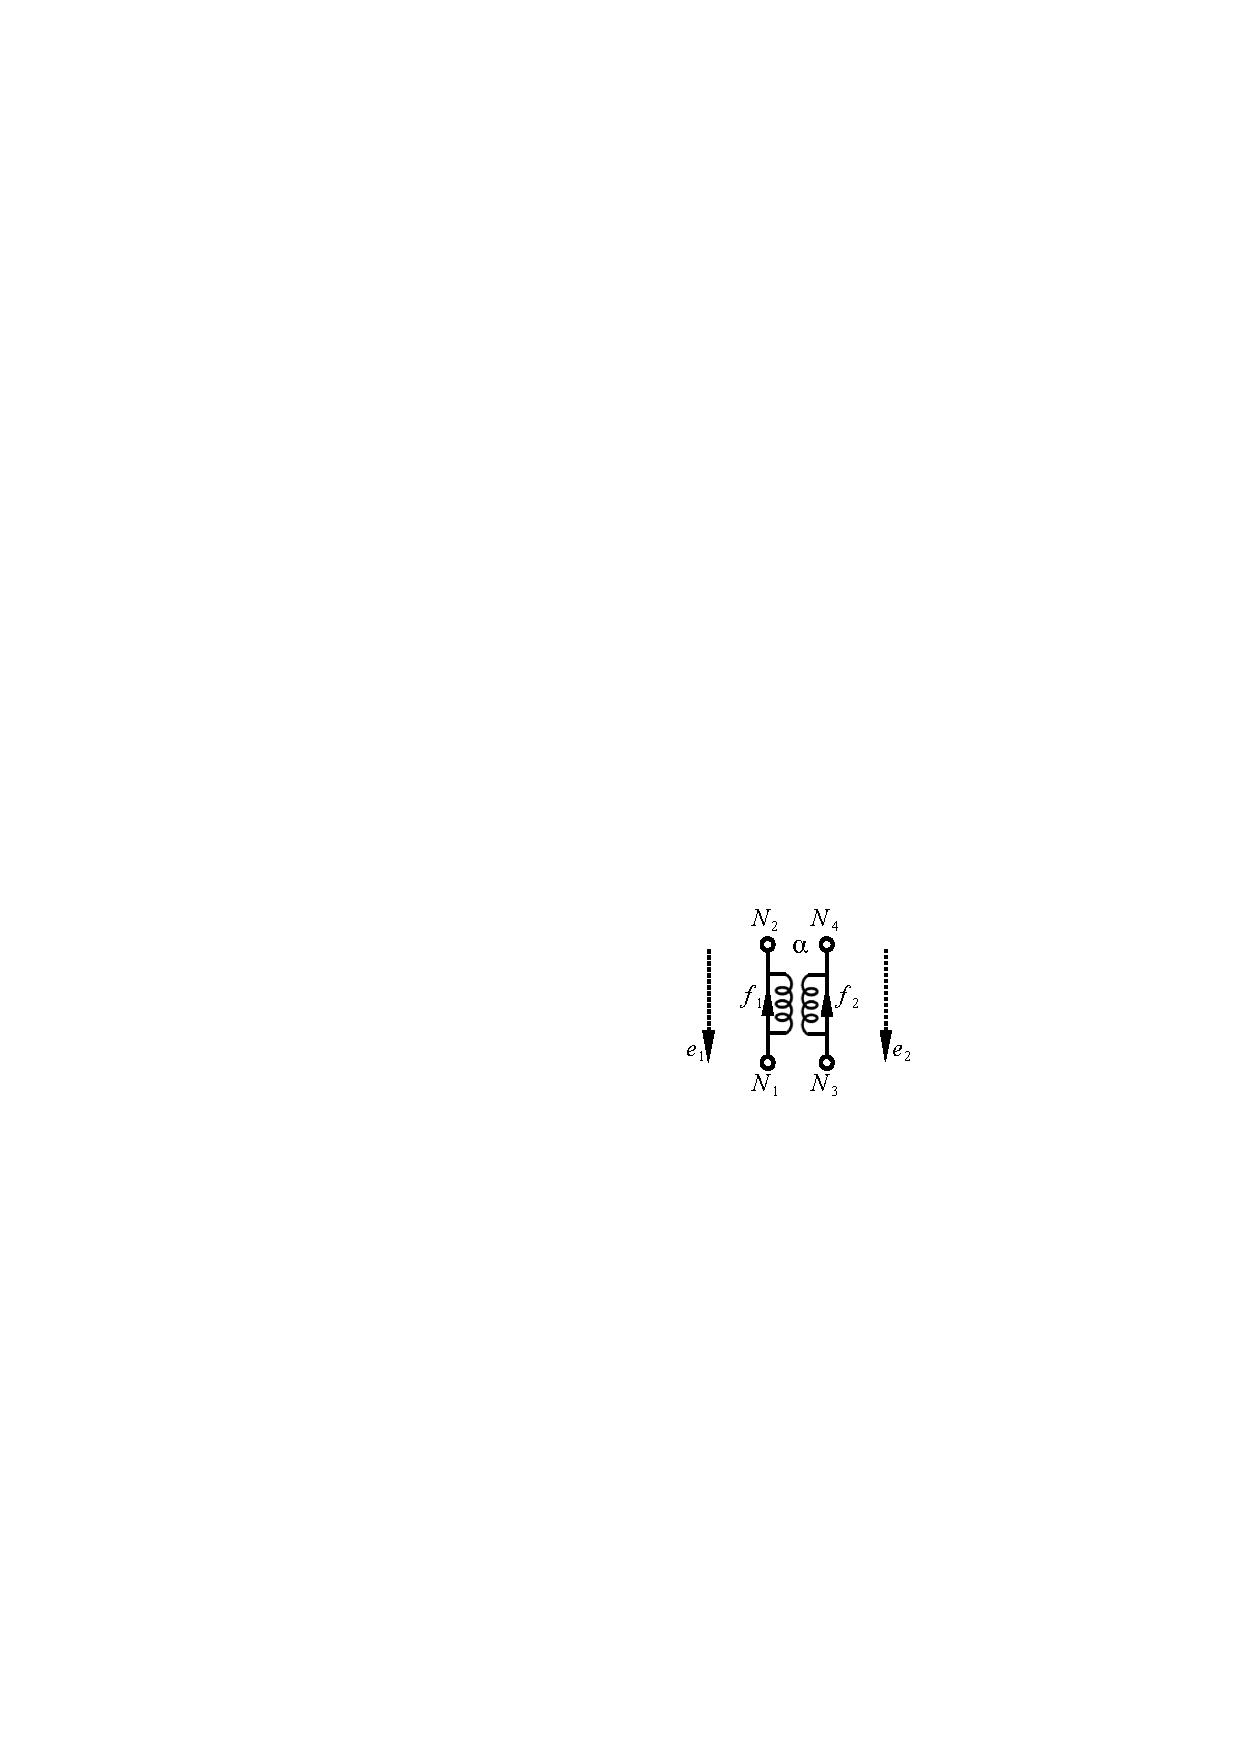
\includegraphics[width=0.3\linewidth]{figures/transformater_scematic.pdf} 
\caption{Scematic and conventions for the transformer.}
\end{figure}
%
\paragraph{Constitutive relations}
$$
\left(
\begin{array}{c}
\e_1\\
\f_2
\end{array}
\right)
=
\left(
\begin{array}{rr}
0 & -\alpha \\
+ \alpha  & 0
\end{array}
\right)
\cdot
\left(
\begin{array}{c}
\f_1\\
\e_2
\end{array}
\right)
$$
%
\section{Fractional calculus}
\label{sec:fractional_calculus}
%
The diffusive process in loudspeakers suspension (creep phenomenon~\ref{pheno:viscoelasticity}) and loudspeakers ferromagnetic path (eddy current phenomenon~\ref{pheno:EddyCurrents}) can be described by linear models that include fractional order dynamics (see \cite{koeller1984applications, lewandowski2010identification, hu2011modal, Holm2013621} for fractional modeling of viscoelasticity, and \cite{schafer2008modelling, laudebat2003modelisation, rumeau2009modelisation} for fractional modeling of eddy currents).
%
A well established formalism for the realization of fractional transfer functions is the so called \emph{diffusive representations}, recalled thereafter (see detailed developements in \cite{helie2006representations,helie2006diffusive}, and \cite{le2012diffusive} for a port-Hamiltonian formulation).
										%
%
%
%
%
%
%
%
%
%
%
%
%
%
%
%
%
%
%
%
%
%
%
\subsection{Fractional integrator}
%
Defining $s \!=\! \rho.e^{i\theta}$, with $\rho\geq 0$ and $\theta \in [-\pi,\pi[$, the transfer function of the fractional integrator $\fracint_\beta(s) = s^{-\beta}$ exhibits a cut $\mathcal{C} =\mathbb{R}_{-}$.
										%
The residue theorem gives the realization of $\fracint_\beta$ as the continuous aggregation of linear damping along the cut $\mathcal{C}$. 
%
This leads to the following \emph{diffusive representation} \cite[\textsection 2]{le2012diffusive}:
%
\begin{equation}
\begin{array}{rcl}
\fracint_\beta(s): \mathbb{C}\setminus\mathbb{R}_{-}&\rightarrow&\mathbb{C}\\
s &\mapsto& \int_0^\infty \mu_\beta(\xi)\frac{1}{s+\xi}\d\xi
\end{array}
\end{equation}
where the weights $\mu_\beta(\xi) = \frac{\fracint_\beta(-\xi-i0^{+})-\fracint_\beta(-\xi+i0^{+})}{2i\pi}=\frac{sin(\beta \pi)}{\pi }\xi^{-\beta}$ correspond to the jump of $\fracint_\beta$ across $\mathcal{C}\equiv\{-\xi\in\mathbb{R}^{-}\}$).										%
%
A state-space representation with output $y_\beta(s) = \fracint_\beta(s) u_\beta(s)$ is:
										%
\begin{equation}
\label{eq:state_frac_int}
\left\{ \begin{array}{cl}
\frac{\d x_\xi}{ \d t} &=  -\xi x_\xi  + u_\beta,\quad x_\xi(0)=0,\\
y_\beta&= \int_0^{+\infty} \mu_\beta(\xi)x_\xi \d \xi .
\end{array} \right.
\end{equation}
										%
The system (\ref{eq:state_frac_int}) is recast as an infinite dimensional pH system (\ref{eq:PHS}), defining the \emph{hamiltonian density }$H_\xi(x_\xi) = \mu_\beta(\xi)  \frac{x_\xi^2}{2} $ and the \emph{resistance density }$r_\xi = \frac{\xi}{\mu_\beta(\xi)}$ with $z_\xi( w_\xi)=r_\xi w_\xi$:
										%
\begin{equation}
\label{eq:phs_frac_int}
\left(\begin{array}{c}
\D{x_\xi}{t}
w_\xi \\
y_\beta
\end{array}\right)
=
\left(\begin{array}{lcc}
0&-1&1\\
1&0&0\\
\ones_\infty&0&0
\end{array}\right)
\left(\begin{array}{c}
\frac{\partial H_\xi}{\d x_\xi}\\
z_\xi( w_\xi) \\
u_\beta
\end{array}\right)
\end{equation}
										%
where $\ones_\infty$ denotes an infinite dimensional row vector of 1, that is $y_\beta = \int_0^{\infty }\frac{\partial H_\xi}{\partial x_\xi} \d \xi$.
%
Notice the total energy is $H_\beta(\mathbf{x}_\beta)\!=\!\int_{\xi\in\mathcal{C}} H_\xi(x_\xi)  \d \xi$ with infinite dimensional state $\bf x_\beta\!\in\!\mathbb{R}^{\mathbb{R_+}}$. 
										%
The realization of the dynamical element with parameter $p$ and transfer function $\fracint_{p,\beta}(s) = (p s^\beta)^{-1}$ is given by (\ref{eq:phs_frac_int}), with $\tilde \mu_{\beta,p}(\xi)= \frac{ \mu_\beta(\xi)}{p}$.
										%
%
%
%
%
%
%
%
%
%
%
%
%
%
%
%
%
%
%
%
%
%
%
\subsection{Fractional differentiator}
\label{sec:frac_diff}
Fractional damping can be modeled as combination of fractional integrators and differentiators (see \cite{koeller1984applications,helie2006diffusive,sabatier2007advances,le2012diffusive}).
%
The realization of fractional differentiator of order $\alpha$ with input $u_\alpha$, transfer function $\fracdiff_\alpha(s)=s^{\alpha}$ and output $y_\alpha=\fracdiff_\alpha u_\alpha$, is built on the diffusive representation (\ref{eq:state_frac_int}) as follows \cite{helie2006diffusive, le2012diffusive}:
%
\begin{equation}
\label{eq:state_frac_diff}
\left\{ \begin{array}{cl}
\frac{\d x_\xi}{ \d t} &=  -\xi\cdot x_\xi  + u_\alpha,\quad x_\xi(0)=0,\\
y_\alpha&= \int_0^{+\infty} \mu_{1-\alpha}(\xi)\big(u_\alpha-\xi\cdot x_\xi)\d \xi .
\end{array} \right.
\end{equation}
%
Defining the \emph{hamiltonian density }$H_\xi(x_\xi) = \mu_{1-\alpha}(\xi) \xi \frac{x_\xi^2}{2} $, the \emph{resistance density }$r_\xi = \mu_{1-\alpha}(\xi)$ and $z_\xi( w_\xi)=r_\xi w_\xi$, the pH formulation of the fractional differentiator (\ref{eq:state_frac_diff}) is 
										%
\begin{equation}
\label{eq:phs_frac_diff}
\left(\begin{array}{c}
\frac{\d x_\xi}{ \d t} \\
w_\xi \\
y_\alpha
\end{array}\right)
=
\left(\begin{array}{lcc}
0 & - \frac{1}{\mu_{1-\alpha}(\xi)} & 0\\
 \frac{1}{\mu_{1-\alpha}(\xi)} & 0 & -1\\
0 & -\ones_\infty & 0
\end{array}\right)
\left(\begin{array}{c}
\frac{\partial H_\xi}{\d x_\xi}\\
z_\xi( w_\xi) \\
u_\alpha
\end{array}\right).
\end{equation}
										%
										%
% 
%
%
%
%
%
%
%
%
%
%
%
%
%
%
%
%
%
%
%
%
%
%
\subsection{Finite order approximation}
\label{sec:Finite_order_approximation}
										%
For implementation purpose, a finite approximation of
diffusive representation (\ref{eq:phs_frac_int}) is built based on a
finite set of $\npoles$ poles ($\xi_1, \dots, \xi_\npoles$) localized on the cut $\mathcal{C}$.
										%
The weights $\bmu=(\mu_1\cdots\mu_\npoles)^T$ are obtained from a least square optimization as detailed in \cite[sec. 5.1.2]{helie2006diffusive}, by minimizing an appropriate distance between $\fracint_\beta$ and its discretisation $\widehat{\fracint}_\beta$:
										%
\begin{equation}
  \label{eq:ApproxHaMatrix}
  \widehat{\fracint}_\beta(s) \!= \sum_{n=1}^\npoles \frac{\mu_n}{s+\xi_n} = \mathbf{E}(s)\cdot \bmu \quad \mbox{with}\quad \mathbf{E}(s)=
  \left(\!
     \begin{array}{c}
      \frac{1}{s+\xi_1} \cdots  \frac{1}{s+\xi_\npoles}
     \end{array}
    \!\right)^\T.
\end{equation}										%
The poles $\xi_n$'s are chosen as $\xi_n  \!= \!\! 10^{\ell_n} \!\in\!\cC,
\mbox{~for~} 
0\!\leq n \leq\! \npoles\!+\!1$,
where the $\ell_n$'s are equally spaced, with step
$\delta\!=\!\frac{\ell_{\npoles+1}-\ell_0}{\npoles\!+\!1}$, from $\ell_0$ to
$\ell_{N+1}$ .
Since gain deviations are perceived relatively to
  the reference gains on the audio range, the weights $\bmu$ are optimized with respect to the objective function
\begin{equation}
  \label{eq:ObjectiveFunction}
  \mathcal{O}(\bmu) = \int_{\omega_{-}}^{\omega_{+}} \left|1-\frac{\widehat{\fracint}_\beta(s\!=\!\Icx\omega)}{{\fracint}_\beta (s\!=\!\Icx\omega)} \right|^2 \mathrm{d}\ln \omega.
\end{equation}
                                %
where $\omega_{-}=2\pi f_{-}$, $\omega_{+}=2\pi f_{+}$ for $[f_{-},f_{+}]=[20\mbox{Hz},\,20\mbox{kHz}]$.
%
In practice, the integral in (\ref{eq:ObjectiveFunction})
is approximated by a finite sum on a frequency grid,
here, $\ln \omega_k\!=\!\ln \omega_{-}\!  +\!  \frac{k}{\nfreqs}
\!\ln\frac{\omega_{+}}{\omega_{-}}$ for $0\!\leq\! k\!\leq\!\nfreqs$.
                                %
This yields the following practical objective function
\begin{equation}
  \widehat{\mathcal{O}}(\bmu) 
=  \herm{(\bf M \bmu - \mathbf{T})}\!  \Wv (\bf M \bmu - \mathbf{T}),
  \label{eq:ObjectiveFunctionNum}
\end{equation}
where matrix $\mathbf M$ is composed of the rows
$[\mathbf M]_{k,:}\!=\!\mathbf E (s\!=\!\Icx\omega_{k-\frac{1}{2}})^T$
defined in~(\ref{eq:ApproxHaMatrix}), where $\omega_{k-\frac{1}{2}}\!=\!\sqrt{
  \omega_{k-1} \omega_k}$ denotes the mean of $\omega_{k-1}$
and $\omega_k$ for $1\!\leq k\!\leq\! \nfreqs$. 
                                %
Vector $\boldsymbol{\fracint}$ is composed of
$[\boldsymbol{\fracint}]_k\!=\!{\fracint}_\beta(s\!=\!\Icx\omega_{k-\frac{1}{2}})$ and
                                %
the diagonal
matrix $\Wv$ is defined by $[\Wv]_{k,k}=(\ln \omega_{k} \!-\! \ln
\omega_{k-1})\,/\, \big|\, [\boldsymbol{\fracint}]_k \big|^2$.
                                %
										%
The minimization of (\ref{eq:ObjectiveFunctionNum}) is achieved by off-the-shelf optimization algorithm, imposing the weights to be positive: 
\begin{equation}
\label{eq:minimization}
 \widehat{\bmu} = \{\min_{\bmu}  \widehat{\mathcal{O}}(\bmu) : \bmu>0\}
\end{equation}
The finite dimensional pH system realizing the weighted fractional integrator with transfer function $\fracint_{p,\beta} = (ps^\beta)^{-1}$ is given in table~\ref{tab:frac_int} with:
										%
\begin{equation}
\label{eq:frac_int_parameters}
\left\{\begin{array}{rcl}
p_n&=&\frac{\widehat{\bmu}_n}{p},\\
r_n&=&\frac{\xi_n}{p_n},
\end{array}\right.\qquad n \in (1,\cdots \npoles).
\end{equation}
%
\begin{table}[h!]
  \centering
  \begin{tabular}[c]{|c|c|}
    \hline
   \begin{minipage}[c|]{5cm}
\vspace{0.2em} \centering  State:\\ $
	\vx_\beta = \left(x_1,\cdots,x_\npoles\right)^\T$
	\\ \vspace{0.2em}
  \end{minipage}
    &\begin{minipage}[c|]{6cm}
\vspace{0.5em} \centering  
Energy:\\ $\H_\beta(\vx_\beta) = \frac{1}{2}\,\vx_\beta^\T\,\diag(p_1,\cdots,p_\npoles)\,\vx_\beta$
\\ \vspace{0.2em}
  \end{minipage}
    \\
    \hline
   \begin{minipage}[c|]{5cm}
\vspace{0.2em}
\centering Dissipation variable:\\ $
	\vw_\beta = \left(w_1,\cdots,w_\npoles\right)^\T
        $\\ \vspace{0.2em}
  \end{minipage}
    &\begin{minipage}[c|]{5cm}
\vspace{0.5em}
\centering
Dissipation law:\\ $\vz_\beta(\vw_\beta) = \diag(r_1,\cdots,r_\npoles)\,\vw_\beta$
\\ \vspace{0.2em}
  \end{minipage}
    \\
    \hline    
    \begin{minipage}[c|]{5cm}
\vspace{0.2em}
\centering
Input:\\
$ u_\beta $\\ \vspace{0.2em} 
  \end{minipage} & \begin{minipage}[c|]{5cm}
\vspace{0.5em}
\centering
Output:\\
$\widehat y_\beta$\\ \vspace{0.2em} 
  \end{minipage}
    \\
    \hline
    \multicolumn{2}{|c|}{
\begin{minipage}[c|]{10cm}
\vspace{0.5em}
\centering
Structure:\\
$\J{xx} = \zeros_{\npoles\times \npoles}$, 
$\J{xw} = -\Id_\npoles$, $\J{xy} =  \ones_{\npoles\times 1}$, \\ $\J{ww}=\zeros_{\npoles\times \npoles}$, $\J{wy}=\zeros_{\npoles\times 1}$, $\J{yy}=0$.
\vspace{0.2em}
  \end{minipage}}
\\
    \hline
  \end{tabular}
  \caption{\label{tab:frac_int} Port-Hamiltonian formulation (\ref{eq:PHS}) for the approximation of the fractional integrator $y_\beta(s)=(p s^\beta)^{-1} u_\beta(s)$ on a finite set of $\npoles$ poles. The parameters $p_n, r_n$ for $n \in (1,\cdots \npoles)$ are defined in (\ref{eq:frac_int_parameters}) based on the minimization of (\ref{eq:ObjectiveFunctionNum}). As an example, if $u_\beta\equiv i$ and $y_\beta \equiv v$, this structure corresponds to the serial connection of $\npoles$ parallel RC cells; if $y_\beta\equiv i$ and $u_\beta \equiv v$, this structure corresponds to the parallel connection of $\npoles$ serial LC cells.}
\end{table}
%
According to section \ref{sec:frac_diff}, the finite dimensional approximation of the weighted fractional differentiator with transfer function $\fracdiff_{\alpha, p} = ps^\alpha$ is obtained from the minimization of (\ref{eq:ObjectiveFunctionNum}) for the transfer function $\fracint_{1-\alpha}$.
%
The corresponding pH formulation is given in table~\ref{tab:frac_diff} with:
										%
\begin{equation}
\label{eq:frac_diff_parameters}
\left\{\begin{array}{rcl}
p_n&=&p\,\widehat{\bmu}_n\,\xi_n,\\
r_n&=&p_n\widehat{\bmu}_n,
\end{array}\right.\qquad n \in (1,\cdots \npoles).
\end{equation}
%
\begin{table}[h!]
  \centering
  \begin{tabular}[c]{|c|c|}
    \hline
   \begin{minipage}[c|]{5cm}
\vspace{0.2em} \centering  State:\\ $
	\vx_\alpha = \left(x_1,\cdots,x_\npoles\right)^\T$
	\\ \vspace{0.2em}
  \end{minipage}
    &\begin{minipage}[c|]{6cm}
\vspace{0.5em} \centering  
Energy:\\ $\H_\alpha(\vx_\alpha) = \frac{1}{2}\,\vx_\alpha^\T\,\diag(p_1,\cdots,p_\npoles)\,\vx_\alpha$
\\ \vspace{0.2em}
  \end{minipage}
    \\
    \hline
   \begin{minipage}[c|]{5cm}
\vspace{0.2em}
\centering Dissipation variable:\\ $
	\vw_\alpha = \left(w_1,\cdots,w_\npoles\right)^\T
        $\\ \vspace{0.2em}
  \end{minipage}
    &\begin{minipage}[c|]{5cm}
\vspace{0.5em}
\centering
Dissipation law:\\ $\vz_\alpha(\vw_\alpha) = \diag(r_1,\cdots,r_\npoles)\,\vw_\alpha$
\\ \vspace{0.2em}
  \end{minipage}
    \\
    \hline    
    \begin{minipage}[c|]{5cm}
\vspace{0.2em}
\centering
Input:\\
$ u_\alpha $\\ \vspace{0.2em} 
  \end{minipage} & \begin{minipage}[c|]{5cm}
\vspace{0.5em}
\centering
Output:\\
$\widehat y_\alpha$\\ \vspace{0.2em} 
  \end{minipage}
    \\
    \hline
    \multicolumn{2}{|c|}{
\begin{minipage}[c|]{10cm}
\vspace{0.5em}
\centering
Structure:\\
$\J{xx} = \zeros_{\npoles\times \npoles}$, 
$\J{xw} = -\diag(\widehat{\bmu})^{-1} $, $\J{xy} = \zeros_{\npoles\times 1}$, \\ $\J{ww}=\zeros_{\npoles\times \npoles}$, $\J{wy}=-\ones_{\npoles\times 1}$, $\J{yy}=0$.
\vspace{0.2em}
  \end{minipage}}
\\
    \hline
  \end{tabular}
  \caption{\label{tab:frac_diff} Port-Hamiltonian formulation (\ref{eq:PHS}) for the approximation of the fractional differentiator $y_\alpha(s)=p s^\alpha\, u_\alpha(s)$ on a finite set of $\npoles$ poles. The parameters $p_n, r_n$ for $n \in (1,\cdots \npoles)$ are defined in (\ref{eq:frac_diff_parameters}) based on the minimization of (\ref{eq:ObjectiveFunctionNum}) for the transfer function $\fracint_{1-\alpha}$. The interpretation is less intuitive than for the fractional integrator of table~\ref{tab:frac_int} due to the coefficients in $\J{xw}$ that involves transformers.}
\end{table}
%
\bibliographystyle{apalike}
\bibliography{documentation}
\end{document}